%******************************************************************************%
%                                                                              %
%                                 Interlude                                    %
%                         for Machine Learning module                          %
%                                                                              %
%******************************************************************************%

% ============================================== %
\section*{Interlude - Plotting Curves With Matplotlib}
% ---------------------------------------------- %

We asked you to plot straight lines in the \texttt{module05}.
Now you are working with polynomial models, the hypothesis functions are not straight lines, but curves.
Plotting curves is a bit more tricky, because if you do not have enough data point, you will get an ugly broken line instead of a smooth curve.
Here's a way to do it.  

Let's begin with a simple dataset:

\begin{minted}[bgcolor=darcula-back,formatcom=\color{lightgrey},fontsize=\scriptsize]{python}
import numpy as np
import matplotlib.pyplot as plt

x = np.arange(1,11).reshape(-1,1)
y = np.array([[ 1.39270298],
           [ 3.88237651],
           [ 4.37726357],
           [ 4.63389049],
           [ 7.79814439],
           [ 6.41717461],
           [ 8.63429886],
           [ 8.19939795],
           [10.37567392],
           [10.68238222]])

plt.scatter(x,y)
plt.show()
\end{minted}

\begin{figure}[!h]
    \centering
    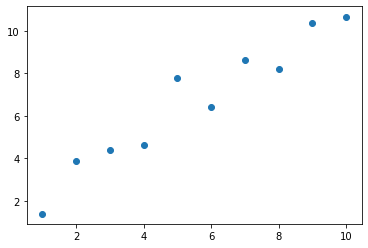
\includegraphics[scale=0.6]{assets/ex12_data.png}
    \caption{Scatter plot of a dataset}
\end{figure}

Now, we build a polynomial model of degree 3 and plot its hypothesis function $h(\theta)$.

\begin{minted}[bgcolor=darcula-back,formatcom=\color{lightgrey},fontsize=\scriptsize]{python}
from polynomial_model import add_polynomial_features
from mylinearregression import MyLinearRegression as MyLR

# Build the model:
x_ = add_polynomial_features(x, 3)
my_lr = MyLR(np.ones(4).reshape(-1,1)).fit_(x_, y)

# Plot:
## To get a smooth curve, we need a lot of data points
continuous_x = np.arange(1,10.01, 0.01).reshape(-1,1)
x_ = add_polynomial_features(continuous_x, 3)
y_hat = my_lr.predict_(continuous_x)

plt.scatter(x,y)
plt.plot(continuous_x, y_hat, color='orange')
plt.show()
\end{minted}

\begin{figure}[!h]
    \centering
    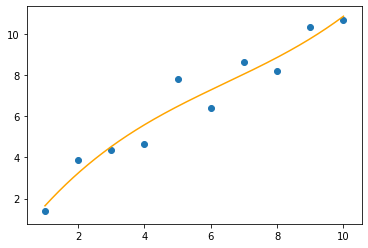
\includegraphics[scale=0.6]{assets/ex12_plot.png}
    \caption{Scatter plot of a dataset, and on top, a plot of the polynomial hypothesis function}
\end{figure}
